% mn2esample.tex
%
% v2.1 released 22nd May 2002 (G. Hutton)
%

\documentclass[useAMS,usenatbib]{mn2e}

\usepackage{graphicx}
\usepackage{verbatim}
\usepackage{natbib}
\usepackage{amsmath}
\usepackage{color}
\usepackage{deluxetable}
\bibliographystyle{mn2e}

%%%%% AUTHORS - PLACE YOUR OWN MACROS HERE %%%%%

%\input blazarenv_macros.tex	
\newcommand{\mnras}{MNRAS}
\newcommand{\apj}{ApJ}
\newcommand{\aj}{AJ}
\newcommand{\apjl}{ApJL}
\newcommand{\apjs}{ApJS}
\newcommand{\aap}{A\&A}
\newcommand{\fcp}{FCP}

%%%%%%%%%%%%%%%%%%%%%%%%%%%%%%%%%%%%%%%%%%%%%%%%

\title[GZ2 data release]{Galaxy Zoo 2: advanced morphological classifications for 304,122 galaxies from the Sloan Digital Sky Survey}
\author[C.J. Lintott, K.W. Willett, etc.]{C. J. Lintott$^{1}$, K. W. Willett$^{2}$, S. P. Bamford$^{3}$, K. L. Masters$^{4}$, B. D. Simmons$^{1,5}$, etc.\\
$^{1}$University of Oxford, UK \\
$^{2}$School of Physics and Astronomy, University of Minnesota, Minneapolis, MN 55455, USA \\
$^{3}$University of Nottingham, UK \\
$^{4}$University of Portsmouth, UK \\
$^{5}$Yale University, New Haven, USA}
\begin{document}

\date{Accepted 1988 December 15. Received 1988 December 14; in original form 1988 October 11}

\pagerange{\pageref{firstpage}--\pageref{lastpage}} \pubyear{2012}

\maketitle

\label{firstpage}

\begin{abstract}
Galaxy Zoo 2 data release paper. 
\end{abstract}

\begin{keywords}
galaxies
\end{keywords}

\section{Introduction} \label{sec-intro}
\section{Project description} \label{sec-description}
\section{Debiasing the data} \label{sec-debias}

\subsection{Using Stripe~82}

One possible method for debiasing the full GZ2 sample is to use the data from Stripe~82 to establish the unbiased level. Normal-depth images for Stripe~82 are selected in precisely the same manner as the main GZ2 sample, with a magnitude limit of $r_{petro} < 17.77$. The fiber size and redshift range are also identically chosen, resulting in a comparison sample of roughly 10\% the size of the GZ2 original + extra samples. 

% From the gz2sample - gz2table match (325651 rows)
% GZ original + extra: no redshifts for 38820/273783 = 14.2%
% GZ s82 normal depth: no redshifts for 3735/21522 =   17.4% 
% GZ s82 coadd1 depth: no redshifts for 10581/30346 =  34.9%
% GZ s82 coadd2 depth: no redshifts for 10578/30339 =  34.9%

Galaxies in Stripe~82 have both ``normal-depth'' images as well as deeper images created by co-adding exposures from the runs that SDSS did in the region prior to DR7 \citep{ann11}. With increased sensitivity to fainter magnitudes, this should mean that galaxies at higher redshifts will have their morphological classifications altered, presumably in the direction of higher accuracy. The spectroscopic incompleteness fraction is similar for the GZ2 original + extra (14\%) and Stripe~82 normal depth (17\%) samples, but is twice as high for the galaxies in the Stripe~82 coadded data (35\%). 

The hypothesis is that the change in vote fraction as a function of galaxy metadata ($z, R_{50}, m_R, \mu$) would have the same effect on classifying GZ2 main sample galaxies at higher redshift in the same $R_{50}, m_R, \mu$ bins. 

Firstly, we need to verify that the distribution of votes for the main sample is similar enough to the Stripe~82 normal-depth (with $r<17.0$) that the same bias correction will apply for both. Table~\ref{tbl-stripe82} shows the tasks in the GZ2 question tree and the mean weighted vote fraction for each response. Overall, the mean values for both the main and Stripe~82 galaxies are very similar, with almost all reponses varying by $<10\%$ between the two samples. The only exceptions to these are for responses that target rare objects (and thus are subject to higher variance for low-number statistics), such as dust lanes, rings, and high-multiplicity spiral arms. 

The right panel of Figure~\ref{fig-task01} shows that the weighted vote fractions also behave similarly as a function of redshift, particularly in the $0.03<z<0.08$ range covered by the GZ1 debiasing technique. The agreement is generally good between the Stripe~82 normal depth and the GZ2 main sample; this is not the case for the coadded Stripe~82 data, however. For Task~01, fewer galaxies are classified as robustly smooth (above the 0.8 threshold), moving instead to the ``unclassified'' category. Similarly, the coadded data shows higher fractions of galaxies with bars (Task~03) and for possessing visible spiral structure (Task~04). A possible cause for this is that the new image pipeline in the coadded data allows viewers to see faint features or disks. The average seeing in the coadded data improves from $1.4\arcsec$ to $1.1\arcsec$ \citep{ann11}, which may need to be corrected for in the Stripe 82 comparisons. 

What needs to be done:
\begin{itemize}
	\item {\bf Yes} Verify that the normal-depth Stripe~82 vote fractions are similar to the original + extra samples. 
	\item {\bf They do, even accounting for the magnitude cut.} See whether co-added images follow a different distribution, esp. as function of $z, R_{50}, M_r, \mu$.
	\item {\bf Only difference is a moderate increase in spiral fraction for disk galaxies in coadd1 data. The results of K-S tests on the weighted vote fractions are confusing. Very similar distributions (by eye) have very low probabilities according to the K-S test.} Decide which of the two co-added samples is more reliable for debiasing efforts
	\item optional: {\it Do a PCA on the normal vs. coadded versions. Figure out which of the four parameters. and in what weighted combination, produces the most scatter in the data. }
	\item How far out in redshift can we correct the normal data using coadd? Need enough galaxies per bin in $M_r$, $R_{50}$, $z$ space {\em for each task} in the Stripe~82 data to establish the baseline. B09 set this at thirty galaxies per bin. 
	\item Figure out how the vote fractions are going to be adjusted once a bias has been identified. 
	\item Apply corrections to the vote fractions in the GZ2 main sample. See if the results are flat for certain tasks (and over what redshift range it applies)
\end{itemize}

\begin{figure*}
\includegraphics[angle=0,width=7.0in]{figures/gz2_bias_demo_task01.ps}
\caption{GZ2 weighted vote fractions for Task 01 ({\it smooth, features/disk, or star/artifact?}) as a function of spectroscopic redshift. The left graph shows the fraction of galaxies for which a category exceeded a threshold of 0.8, including galaxies which had no answer above the threshold. The right shows the mean of the vote fractions, weighted by the total number of responses to the task for each galaxy. Data are shown for the GZ2 original + extra (thick), Stripe~82 normal-depth (thin dotted), and Stripe~82 co-add depth (thin solid) samples. Stripe~82 data is only for galaxies with $r < 17.0$, the same magnitude limit applied to the GZ2 main sample.  
\label{fig-task01}}
\end{figure*}


\section{The catalog} \label{sec-catalog}

\section{Comparison of GZ2 to other classification methods}\label{sec-comparison}

\begin{itemize}
	\item \citet{nai10}
	\item \citet{hue11}
	\item CAS studies \citep{con03,con06} 
	\item EFIGI \citep{bai11}
\end{itemize}

The main purpose of this section is to perform preliminary comparisons between the weighted, but not debiased data from GZ2 available in early 2012. This analysis will need to be repeated to account for biases in the data; hopefully with the groundwork laid here, it will be faster to repeat it later.  

\subsection{Nair \& Abraham}

\citet[][; hereafter NA10]{nai10} catalogued 14,034 galaxies from the SDSS DR4. The galaxy redshifts range from $0.01<z<0.1$, and go down to an extinction-corrected apparent magnitude limit of $g<16$. Overlap with the GZ2 sample is substantial; joining on their objIDs, 12,480 galaxies are found in both catalogs. This comprises 89.9\% of the NA10 catalog, but only 4.5\% of the total GZ2 sample. The GZ2 sample is deeper ($r<17$), spans a wider redshift range ($0.0005<z<0.25$), and contains more recent data releases (DR7) than the NA10 catalog. 

\citet{nai10} used classifications by a single professional (P. Nair) to carry out morphological classifications. She determined RC3 T-Types for the entire sample through visual inspection of $g$-band images, covering each source twice. There is no discussion as to the procedure if T-Types changed between her first and second classifications. 

In addition to the T-Types, she also classified various ``fine structure'' morphological features in each galaxy. It is not stated how many times these classifications were performed. These include:

\begin{itemize}
	\item bars (strong, weak, intermediate, ansae, ``peanut'', nuclear, and/or unsure)
	\item rings (nuclear, inner, outer)
	\item lenses [regions of constant surface brightness; NOT gravitational lenses] (inner, outer)
	\item pairs of objects (close, projected, adjacent, overlapping, + flags for second object type)
	\item interaction (none, disturbed, warp, shells, short tail, medium tail, long tail, bridge)
	\item tails (number)
\end{itemize}

Several of the fine structure features can be directly compared to the GZ2 data: bars, rings, and pairs/interactions. 

\subsubsection{Bars}

NA10 detect 2537 barred galaxies, which is 18\% of their total sample. For objects with T-Types later than E/S0, this rises to 25\% of the sample. This is much lower than the fraction found in local galaxies ($\sim60\%$), but similar to the fraction found by \citep{mas11c} for the bar fraction in disky, face-on galaxies from GZ2 (29.4\%). 

\begin{figure*}
\includegraphics[angle=-90,width=7.0in]{figures/na_bars_axial_10.ps}
\caption{NA10 bar classifications compared to GZ2. Data are for the 7,121 galaxies which are face-on (log~$(a/b)<0.3$) and with 10 or more GZ2 bar classifications. 
\label{fig-na_bars}}
\end{figure*}

Two parameters can be set that reduce the number of galaxies in the overlap between the samples, but result in a cleaner cut for comparisons. The first uses the \citet{mas11c} cut for face-on galaxies (log~$(a/b) < 0.3$ using the {\tt expab\_r} parameter in the Galaxy table). The second is to only look at galaxies with at least 10 classifications for task 03 ({\it bar present?}) in GZ2. The reduced face-on sample has 7,121 galaxies from the original 12,480. All trends described below hold generally for both the full overlapping samples and the cleaner face-on sub-sample.

Of the objects NA10 identify as barred, 2348/2537 (93\%) are objects in GZ2. Figure~\ref{fig-na_bars} shows correlations for face-on galaxies between the bar fractions of the NA10 and GZ2 catalogs. Galaxies in NA10 are classified by a single person, and so the presence of a bar is indicated with a series of flags. Bars in a galaxy can be classified according to strength (weak, intermediate, strong) or by other morphological features (ansae, peanuts, or nuclear bar). A galaxy may in rare cases have both a disk-scale (strong, intermediate, or weak) and a nuclear bar. 

Figure~\ref{fig-na_bars} shows that the raw GZ2 weighted bar fraction (WBF) very closely agrees with the NA10 fraction of barred galaxies for each GZ2 bin. The two quantities are not identical; the x-axis plots galaxies with {\it individual classifications} at whatever fraction of votes chose a bar. The y-axis shows that for galaxies in that WBF bin from GZ, the average bar classification is similar to the weighted vote totals. The distribution shows a Spearman's rho of $\rho=0.984$, and closely follows a 1:1 relationship between the two lines. If supported by debiased GZ2 data, this means that the aggregate votes of Zooites closely reproduce the expert classification of NA10. 

In the top right, Figure~\ref{fig-na_bars} shows the distribution of GZ2 bar votes by simply splitting the NA10 sample in two: galaxies without a bar and galaxies with a bar (of any kind). Both samples show a strong trend toward either extrema, although there are a large number of galaxies in GZ2 with a fraction of 0.0 than one would expect. Possession of a bar is less straightforward; while the frequency of NA10 bars does increase with GZ2 fraction, 32\% of NA-barred galaxies lie below the canonical GZ2 WBF of 0.5. Conversely, there are very few false positives (5.5\% of non-barred NA10 galaxies) above this value. 

In the bottom left of Figure~\ref{fig-na_bars}, the distribution of GZ2 WBF as a function of NA10 bar strength is plotted. The distribution for all bars is the same as shown in the top right, increasing with GZ2 WBF. There is a clear difference in GZ classification between the three sets of bars; interestingly, all three are statistically highly distinct from each other and from the overall barred sample, according to a two-sided K-S test. The majority of both the strong and intermediate barred population have high GZ2 WBFs, with 83\% of strong bars and 56\% of intermediate bars above a bar fraction of 0.8. Those numbers increase to 98\% and 90\%, respectively, if the criterion of 0.5 for the GZ2 WBF is used \citep{mas11c}. Weakly-barred galaxies have only 13\% of their GZ2 WBFs above 0.8 and 47\% above 0.5. 

NA10 identify three other fine-structure features related to bars: ansae, peanuts, and nuclear bars. None of the three correlate strongly with a high GZ2 WBF, with most galaxies in all three features at less than 0.5. Nuclear bars are the only feature that overlaps with the NA10 bar classifications; out of 283 nuclear bars, 3 galaxies also have strong bars, 44 have intermediate bars, and 166 have weak bars. No ansae are detected in the face-on subsample of galaxies, due to the axial cut. 

\begin{figure*}
\includegraphics[angle=-90,width=7.0in]{figures/na_rings_axial.ps}
\caption{NA10 ring classifications compared to GZ2. Data are for the 9,746 galaxies in both samples which are face-on (log~$(a/b)<0.3$). 
\label{fig-na_rings}}
\end{figure*}

In the full GZ2 sample (original + extra), 87,651 galaxies had at least 10 responses to the question {\it ``Is there a sign of a bar feature?''}  - 22.1\% of them had a WBF greater or equal to 0.5. In the clean face-on sample, this rises to 28.7\%.This is in very good agreement with both the 29.4\% fraction found in the smaller volume-limited sample of \citet{mas11c}, and with the $\sim30\%$ for disk galaxies with $(b/a)>0.4$ (or log~$(a/b)<0.398$) and T-types of S0 or later of \citet{nai10a}. 

In the published literature, \citep{mas11c} mention the NA10 catalog and note that both papers agree with a bar fraction depending on morphology with a minimum near the division between the blue and red sequences. There is no detailed comparison between the galaxies in the two samples.

\subsubsection{Rings}

The NA10 catalog also classifies ring galaxies in their sample. They include three basic types of rings in the catalog \citep{but96}. Inner rings lie between the bulge and spiral arms or disk. Outer rings are external to the spiral arms, but are still closely linked to the spiral pattern. Nuclear rings lie in the bulge region of galaxies; no specific size scale for this is given. In GZ2, rings are classified only if the user answers ``Yes'' to the question {\it ``Anything odd?''} Since the user then has six different options to choose from (ring, lens, disturbed, irregular, other, merger), the weighted ring fractions is less straightforward than for a binary tree. 

In the NA10 catalog, 18.2\% of galaxies have a ring. Of those, 10\% are nuclear rings, 74\% are inner rings, and 32\% are outer rings (sum is more than 100\% since $\sim1/3$ of ringed galaxies have multiple rings flagged). In the GZ2 catalog, 8.2\% of galaxies have at least 10 votes for a ring, while 22\% (10\%) have a weighted fraction higher than 0.5 (0.8). In both catalogs, selecting only face-on galaxies makes no significant changes in the percentage of galaxies identified as having a ring. 

In the top-left of Figure~\ref{fig-na_rings}, the distribution of the number of GZ2 votes for a ring in face-on galaxies is shown, both for the total sample and for galaxies classified by NA10 as having a ring. The distributions grow closer as the number of ``Yes'' votes increases. The top-right panel of Figure~\ref{fig-na_bars} shows the CDF for the number of ring votes. Among all galaxies with at least 15 ``Yes'' votes, for example, $\sim90\%$ of those galaxies are also identified by NA10 as having a ring; almost all of these are inner or outer rings.  

In contrast, the weighted ring fraction (WRF) from the GZ2 votes is not a good match to the ring classifications of NA10. Half of all galaxies have a WRF of 0.0, indicating no votes for a ring-like structure in the image. For ringed galaxies identified by NA, the number of WRF=0.0 objects decreases dramatically, but results a generally flat distribution of ring fractions. No single cut on WRF is a good proxy for the NA10 classifications; at all WBF above 0.5, for example, only $\sim45-65\%$ of the GZ2 ringed galaxies are identified as rings in NA10.  

There is some evidence indicating that GZ2 classifications are sensitive only to certain types of rings. NA10 galaxies with nuclear rings, for example, have a large number of galaxies with no GZ2 ring votes. Several causes are possible: since nuclear rings are smaller, they are more difficult to discern in low surface brightness or bulge-dominated galaxies. In addition, the button in the GZ2 tree intended to show an example of a ring has a center dot (presumably a galactic bulge) surrounded by a ring. This could reasonably represent either an inner or outer ring, but would presumably not be associated with the intra-bulge nuclear rings by an untrained user. The bottom-right panel of Figure~\ref{fig-na_rings} shows that the number of NA10 galaxies with inner and/or outer rings does rise with WRF, but is still only 55\% successful at WRF$ > 0.8$. 

\subsubsection{Mergers/interacting galaxies}

\begin{figure*}
\includegraphics[angle=-90,width=7.0in]{figures/na_pairs.ps}
\caption{NA10 galaxies as a function of the votes/vote fraction for merger in GZ2. This includes all galaxies in the overlap sample (black), galaxies in pairs (blue), and interacting galaxies (red). Data are for the 12,480 galaxies found in both samples.
\label{fig-na_pairs}}
\end{figure*}

Galaxies in GZ2 can be labeled as a ``merger'' under the task {\it ``Anything odd?''} NA10 classify possible mergers in two ways: by identifying pairs of objects in an image, and by identifying interacting galaxies. Both NA10 categories have sub-levels: paired objects are sorted by relative separation (close, projected, apparent, or overlapping pairs), and interactions by morphology (disturbed, warp, shells, tails, or bridges). If tidal tails are present, there is an additional flag couting the number of tails. 

In the NA10 catalog, 22.3\% of galaxies are labeled as paired; of these, the majority (72\%) are close pairs. Interacting galaxies are a much smaller subset, comprising 7\% of the NA10 sample. In the GZ2 catalog, only 3.6\% (1.8\%) of galaxies have a merger weighted fraction above 0.5 (0.8). If the vote totals for a possible merger are used instead, 5\% (3\%) of galaxies have at least 5 (10) votes for a merger. The large fraction of NA10 galaxies suggests that this is less likely to be a good proxy for a merger as identified by the GZ2 votes; interacting galaxies may be a more promising proxy. 

Figure~\ref{fig-na_pairs} shows the distributions of NA10 paired and interacting galaxies. Most galaxies in the overlapping sample have no votes for a merger; the same trends are seen for both pairs and interactions. If using the raw number of votes as a cutoff, GZ2 galaxies stabilize at an 80\% match rate to the NA10 paired galaxies for 8 or more merger votes. The trend for interacting galaxies continues to increase with higher numbers of votes, only matching the 80\% level at 25 or more merger votes, for which less than 100 galaxies are included.

Using the weighted merger fraction instead of the raw vote counts does not show a strong correlation with the NA10 classifications. Interestingly, both show peaks if a weighted merger fraction cutoff of 0.5 is chosen. The peak of the NA10 fraction, however, is significantly lower if matching on the weighted merger fraction; only 70\% for paired galaxies and 40\% for interacting galaxies. This shows no difference depending on the type of NA10 pair. Within the NA10 interacting classes, all actually show a decrease in number for a higher weighted merger fraction; the only exception is galaxies classified as bridges, the fraction of which increases slightly above a weighted merger fraction of 0.5. 

Similar to the results above, there is no strong correlation between either the GZ2 weighted merger fraction or number of merger votes and the number of NA-identified tidal tails. 

\subsubsection{T-types}

There has been no published discussion in the literature comparing large-scale morphologies of the NA10 and GZ catalogs. \citet{nai10} was published after the first GZ1 results, \citep{lin08}, but prior to the formal data release paper \citep{lin11}. \citet{hue11} do compare automated classifications to both NA10 and GZ1, finding good agreement with both; this obliquely suggests that the GZ2 and NA10 classifications will also be consistent. 

\begin{figure*}
%\includegraphics[angle=-90,width=7.0in]{figures/na_ttype.ps}
\includegraphics[angle=0,width=7.0in]{figures/na_ttype.eps}
\caption{NA10 T-Type classifications compared to GZ2. Data on the left are for the 12,480 galaxies found in both samples; the right only shows the 5,683 galaxies with at least 10 responses to Task 04 (visible spiral structure) in GZ2. 
\label{fig-na_ttype}}
\end{figure*}

The left panel of Figure~\ref{fig-na_ttype} shows the percentage of galaxies identified as having either a disk or features from the first question in the GZ2 tree, color-coded by their NA10 T-Types. There is a clear separation in the GZ2 fractions for galaxies classified as E vs. those with T-Types Sa and later. Late-type galaxies, including S0's, have a median weighted fraction of the ``features or disk question'' of 0.796, with a standard deviation of 0.29. This distribution is bimodal, with one peak near 0.95 and a second at 0.1. Breaking down the late-type galaxies into more specific Hubble classifications, the late-type galaxies with low GZ2 feature votes are found to be primarily lenticular (S0; T-Type = -3 to 0) galaxies. If only galaxies with T-Types Sa or later are considered, the peak at lower GZ2 fractions disappears. The median GZ2 weighted fraction for these galaxies is 0.88, with a standard deviation of 0.23. The highest GZ2 weighted fraction for an elliptical galaxy in NA10 is 0.741; therefore, any cut above this limit includes {\it exclusively} identified by NA10 as late-type. Even if the confidence of this decreases for the larger GZ2 sample due to the inclusion of fainter galaxies, the previous limit of 0.8 (which may be conservative) reproduces the broad morphological cuts of NA10 extremely well. 

Since there are very few objects identified as stars or artifacts in the first GZ2 question, the weighted fraction for smooth galaxies is approximately $f_{smooth} = (1 - f_{features\_or\_disk})$. Elliptical galaxies (T-Type = -5) have a median weighted fraction of the ``smooth'' question of 0.86, with a standard deviation of 0.07. The GZ2 votes for the NA10 ellipticals are much more sharply peaked than the late-type galaxies, lacking the long tail seen even for very late types. This means that a cut on GZ2 votes for smooth galaxies at 0.8, for example, would include 4\% late-type galaxies (20\% if S0 galaxies are included). 

For galaxies identified as having features that are not edge-on disks, GZ2 users then vote on whether the galaxy has visible spiral structure (Task 04). For the few NA10 elliptical galaxies that have votes for this question, $\sim85\%$ of them have GZ2 weighted fractions of 0.0, with the remainder weakly clustered around 0.3. For NA10 late-type galaxies, the majority of disk/feature objects have high GZ2 spiral structure weighted fractions. For galaxies with at least 10 votes on Task 04 (a peak at 0.0 appears when this cut is not imposed), 70\% of Sa or later-types have a GZ2 spiral vote above 0.8. This drops to 60\% if S0 galaxies are included as late-type. The missing population is thus made up of galaxies with significant spiral structure by NA10, but for which GZ2 users cannot distinguish spiral arms. One might expect these galaxies to have lower magnitudes or surface brightnesses compared to the rest of the sample, thus lowering the confidence of GZ2 votes (there is no analog parameter associated with NA10 classifications). However, the apparent $g$ and $r$ magnitudes, as well as the absolute $g$-band magnitude, show no difference between galaxies above and below the 80\% cutoff. Experimenting with other values for the GZ2 weighted fraction had no change on the results.  

\subsubsection{Spiral tightness}

\begin{figure*}
\includegraphics[angle=-90,width=7.0in]{figures/spiraltightness_color.ps}
\caption{T-Type classifications compared to the GZ2 vote fractions for spiral tightness (Task 10). Left side is NA10 T-Types; right side is EFIGI T-Types. Data are for the 5,515 (NA10) and 1,907 (EFIGI) galaxies, respectively, with at least 10 GZ2 votes for Task 10. The number of galaxies per bin is indicated along the top of each panel. 
\label{fig-spiraltightness}}
\end{figure*}

If a disk galaxy was identified as having spiral structure, Task~10 in GZ2 asked users to classify the ``tightness' of the spiral arms. This task had three options: tight, medium, or loose (accompanied with pictograms on buttons that illustrated representative pitch angles). This has direct (but not exclusive) connections to the Hubble classification of late-type galaxies; tight spirals would be Sa/Sb, medium spirals Sb/Sc, and loose spirals Sc/Sd. The agreement between the GZ2 classification can be compared to Hubble types by using the NA10 classifications. 

The left side of Figure~\ref{fig-spiraltightness} shows the distribution of NA10 T-Types for galaxies based on their GZ2 weighted fractions for winding arms. This figure shows only galaxies with at least 10 votes on spiral structure; looking at all galaxies in the overlapping sample disproportionally weights the 0.0 and 1.0 weighted fraction bins. Weighted fractions for both tight and medium winding arms are relatively normally distributed, with tight spirals peaking near 0.46 and medium spirals at 0.37. Strongly-classified loose spirals are much rarer, with 75\% of galaxies having a weighted fraction of less than 0.2. Almost no elliptical galaxies from the NA10 catalog are included, although there are significant numbers of S0 galaxies. 

For tight spirals, galaxies with the highest weighted fractions have more earlier-type spirals than galaxies with a low vote for tight spiral winding arms. For a tight spiral weighted fraction above 0.9, 85\% of galaxies are Sb or earlier. Medium-wound spirals with high weighted fractions tend to be Sb and Sc galaxies -- the proportion of both types increases as a function of medium-wound weighted fraction, and constitute 84\% of galaxies when the weighted fraction is greater than 0.6. Galaxies strongly classified as medium-wound are rare, however, with only 23 galaxies having a weighted fraction above 0.8.  Loose spirals are dominated by Sc and Sd galaxies at high weighted fraction values, comprising more than 50\% of galaxies above a loose weighted fraction of 0.7. 

Overall, we see a clear trend for looser GZ2 spiral arms to correspond with later spiral T-Types from NA10 classifications. High weighted vote fractions are mostly Sa/Sb galaxies for tight winding, Sb/Sc galaxies for medium winding, and Sc/Sd galaxies for loose winding. Individual GZ2 vote fractions, however, have significant diversity even at the highest bins, and do not reliably separate the morphologies on the level of the Hubble T-Types. 

%It would be potentially useful to try combining the winding arms classifications to improve the 40\% false positive rate; for example, by seeing if a high value for loose weighted fraction + a low value for a tight weighted fraction increased the fraction of Sc and Sd galaxies in the highest bins. 

\subsubsection{Bulge dominance}

\begin{figure*}
\includegraphics[angle=-90,width=7.0in]{figures/bulgeprominence_color.ps}
\caption{T-Type classifications compared to the GZ2 vote fractions for bulge prominence (Task 05). Left side is NA10 T-Types; right side is EFIGI T-Types. Data are for the 7,120 (NA10) and 2,321 (EFIGI) galaxies, respectively, with at least 10 GZ2 votes for Task 05. The number of galaxies per bin is indicated along the top of each panel. 
\label{fig-bulgeprominence}}
\end{figure*}

\begin{figure*}
\includegraphics[angle=-90,width=7.0in]{figures/wbulge_wspiral.ps}
\caption{Weighted bulge classifications vs. weighted spiral classifications from GZ2. Galaxies are color-coded by their morphologies in EFIGI ({\it top}) and NA10 ({\it bottom}). Data are for galaxies with at least 10 classifications for both Task 05 (bulge dominance) and Task 10 (spiral structure) in GZ2. 
\label{fig-bulgespiral}}
\end{figure*}

Disk galaxies in GZ2 are also classified by the a visible dominance of a bulge (Task~05), irrespective of whether spiral structure is also identified. This task has four options: ``no bulge'', ``just noticeable'', ``obvious'', and ``dominant'' (accompanied with pictograms that illustrated bulge sizes compared to face-on spiral arms). Similar to the arm tightness task, we analyze the relationships between GZ2 classification and Hubble types from NA10. 

The left side of Figure~\ref{fig-bulgeprominence} shows the distribution of NA10 T-Types for galaxies based on their GZ2 weighted fractions for winding arms. This figure shows only galaxies with at least 10 votes on bulge prominence. Weighted fractions for both the ``no bulge'' and ``dominant'' responses peak strongly near zero and tail off as the vote fraction increases. Responses to the middle options, ``just noticeable'' and ``obvious'', resemble normal distributions peaking near 0.5. 

``No bulge'' galaxies in GZ2 are dominated by Sc and Sd spirals for non-zero weighted fractions. For weighted fractions above 0.1, 81\% of galaxies are Sc or later; this rises to 100\% for weighted fractions higher than 0.6. ``Just noticeable'' galaxies show a smooth change in T-Type distribution; low weighted fractions are dominated by S0 and Sa galaxies, while high weighted fractions are Sb-Sd. ``Obvious'' bulge galaxies are almost a mirror image of the ``just noticeable'' votes; low weighted fractions are Sb--Sd galaxies, and high weighted fractions are S0--Sa galaxies. Among galaxies classified as ``dominant'', less than 10 galaxies have weighted fractions above 0.6 (which are a surprisingly diverse mix of S0, Sa, and Sd). Most remaining galaxies have dominant weighted fractions of less than 0.1; the T-Types of the remaining galaxies between 0.1 and 0.6 mostly contain S0 and Sa spirals. 

The link to T-Type is more sharply defined for bulge prominence than for spiral tightness, according to the NA10 classifications. Very clean samples of late-type (Sb--Sd) spirals can be selected using only the ``no bulge'' parameter; additional samples with $\sim10$\% contamination can be selected with the ``just noticeable'' and ``obvious'' distributions. Early-type spirals and lenticulars at the same purity level can also be selected. Elliptical galaxies for which the bulge question was answered are most often ``dominant'', but there is no obvious separation of ellipticals from disk galaxies based on this task. 

Since Hubble types are based on both bulge dominance and the distance of their spirals, we explore whether the combination of Tasks 05 and 10 from GZ2 improve the separation between T-Types. Figure~\ref{fig-bulgespiral} shows the GZ2 bulge prominence vs. spiral tightness, color-coded by their NA10 T-Types. The GZ2 variables are a weighted average of the votes for all possible task responses, where:

\begin{eqnarray}
\label{eqn-wbulge}
p_{bulge} = (0f_{nobulge} + 1f_{justnoticeable} \\
            + 2f_{obvious} + 3f_{dominant}) / 3., \nonumber
\end{eqnarray}

\noindent and 

\begin{equation}
\label{eqn-wspiral}
p_{spiral} = (0 \times f_{tight} + 1 \times f_{medium} + 2 \times f_{loose}) / 2.
\end{equation}

Using the weighted feature classifications shows a clear separation in T-Types; the majority of this, however, is for the bulge prominence category. Spiral prominence does not seem to significantly affect any of the classifications. 

\subsubsection{T-Types to clicks}

\begin{itemize}
	\item How like a given T-Type is a galaxy?
	\item Take all GZ2 vote fractions, plus galaxy metadata ($z, R_{50}, m_R, \mu$)
	\item Run a PCA on NA10 classifications to see which GZ2 parameters are most important
	\item Apply it and get the likelihood of a particular galaxy from the ~20 axes
	\item This is the training set that is applied to the rest of Zoo2, accounting for evolution in the metadata properties on which the PCA can act.
\end{itemize}

\subsection{EFIGI}

\citet{bai11} performed individual morphological classifications of 4,458 galaxies for EFIGI (Extractions de Formes Id\'ealis\'ees de Galaxies en Imagerie). The sample is a subset of the RC3 catalog for which 5-color imaging in the SDSS DR4 was available. Images are supplemented by redshift information from several different sources. The galaxies have no strong redshift or volume limit on the sample, with almost all galaxies at $0.0001<z<0.08$. Classifications on composite $gri$ images were performed by a group of 11 astronomers, each of whom classified a subset of 445 galaxies. A training set of 100 galaxies was classified by all astronomers in the group to adjust for individual bias. 

EFIGI contains two types of morphological classification: T-Types and attributes. T-Types are assigned using a slightly modified version of the RC3 Hubble classifications. Peculiar galaxies are not considered a separate stage, and ellipticals are subdivided into various types: compact, elongated (standard elliptical), cD (giant elliptical), and dwarf spheroidals. They also classify late-type lenticulars (S0$^+$; T-Type=-1) that are not included in the classification of NA10. The remaining morphological information, called attributes, is divided into six groups:

\begin{itemize}
	\item appearance: {\tt inclination/elongation }
	\item environment: {\tt multiplicity, contamination}
	\item bulge: {\tt B/T ratio}
	\item spiral arms: {\tt arm strength, arm curvature, rotation}
	\item texture: {\tt visible dust, dust dispersion, flocculence, hot spots}
	\item dynamics: {\tt bar length, inner ring, outer ring, pseudo-ring, perturbation}
\end{itemize}

\noindent Attributes are defined on a five-step scale from 0 to 1 (0, 0.25, 0.50, 0.75, 1) that describe the strength of the feature in question. For some attributes (eg, arm strength, rings), the scale is set by the fraction of the flux contribution of the feature relative to that of the entire galaxy; this scale may not be linear. For others (eg, inclination or multiplicity), it ranges between the extrema of possible values. A 70\% confidence interval (roughly 1$\sigma$) is estimated by setting lower and upper limits on the same five-point scale.

EFIGI is compared in detail to NA10 in \citet{bai11}. Only $\sim10\%$ of the NA10 catalog overlaps with EFIGI classifications; roughly one-third of the EFIGI sample lies at redshifts below the NA10 lower limit of $z=0.01$, and also contain significant number of galaxies fainter than $g=16$. T-Types agree well between the two samples; EFIGI lenticular and early spirals have slightly later average classifications in NA10, while later EFIGI galaxies have slightly earlier NA10 T-Types. EFIGI has a major fraction of galaxies with slight-to-moderate perturbations that have no interaction flags in the NA10 catalog, indicating that NA10 is less sensitive toward more benign features (eg, spiral arm asymmetry). The bar length scale is consistent between the two samples; good agreement is also found for ring classifications. 

3,411 galaxies appear in both EFIGI and GZ2. This constitutes 77\% of the EFIGI galaxies and 1.2\% of the GZ2 sample. 

\begin{figure*}
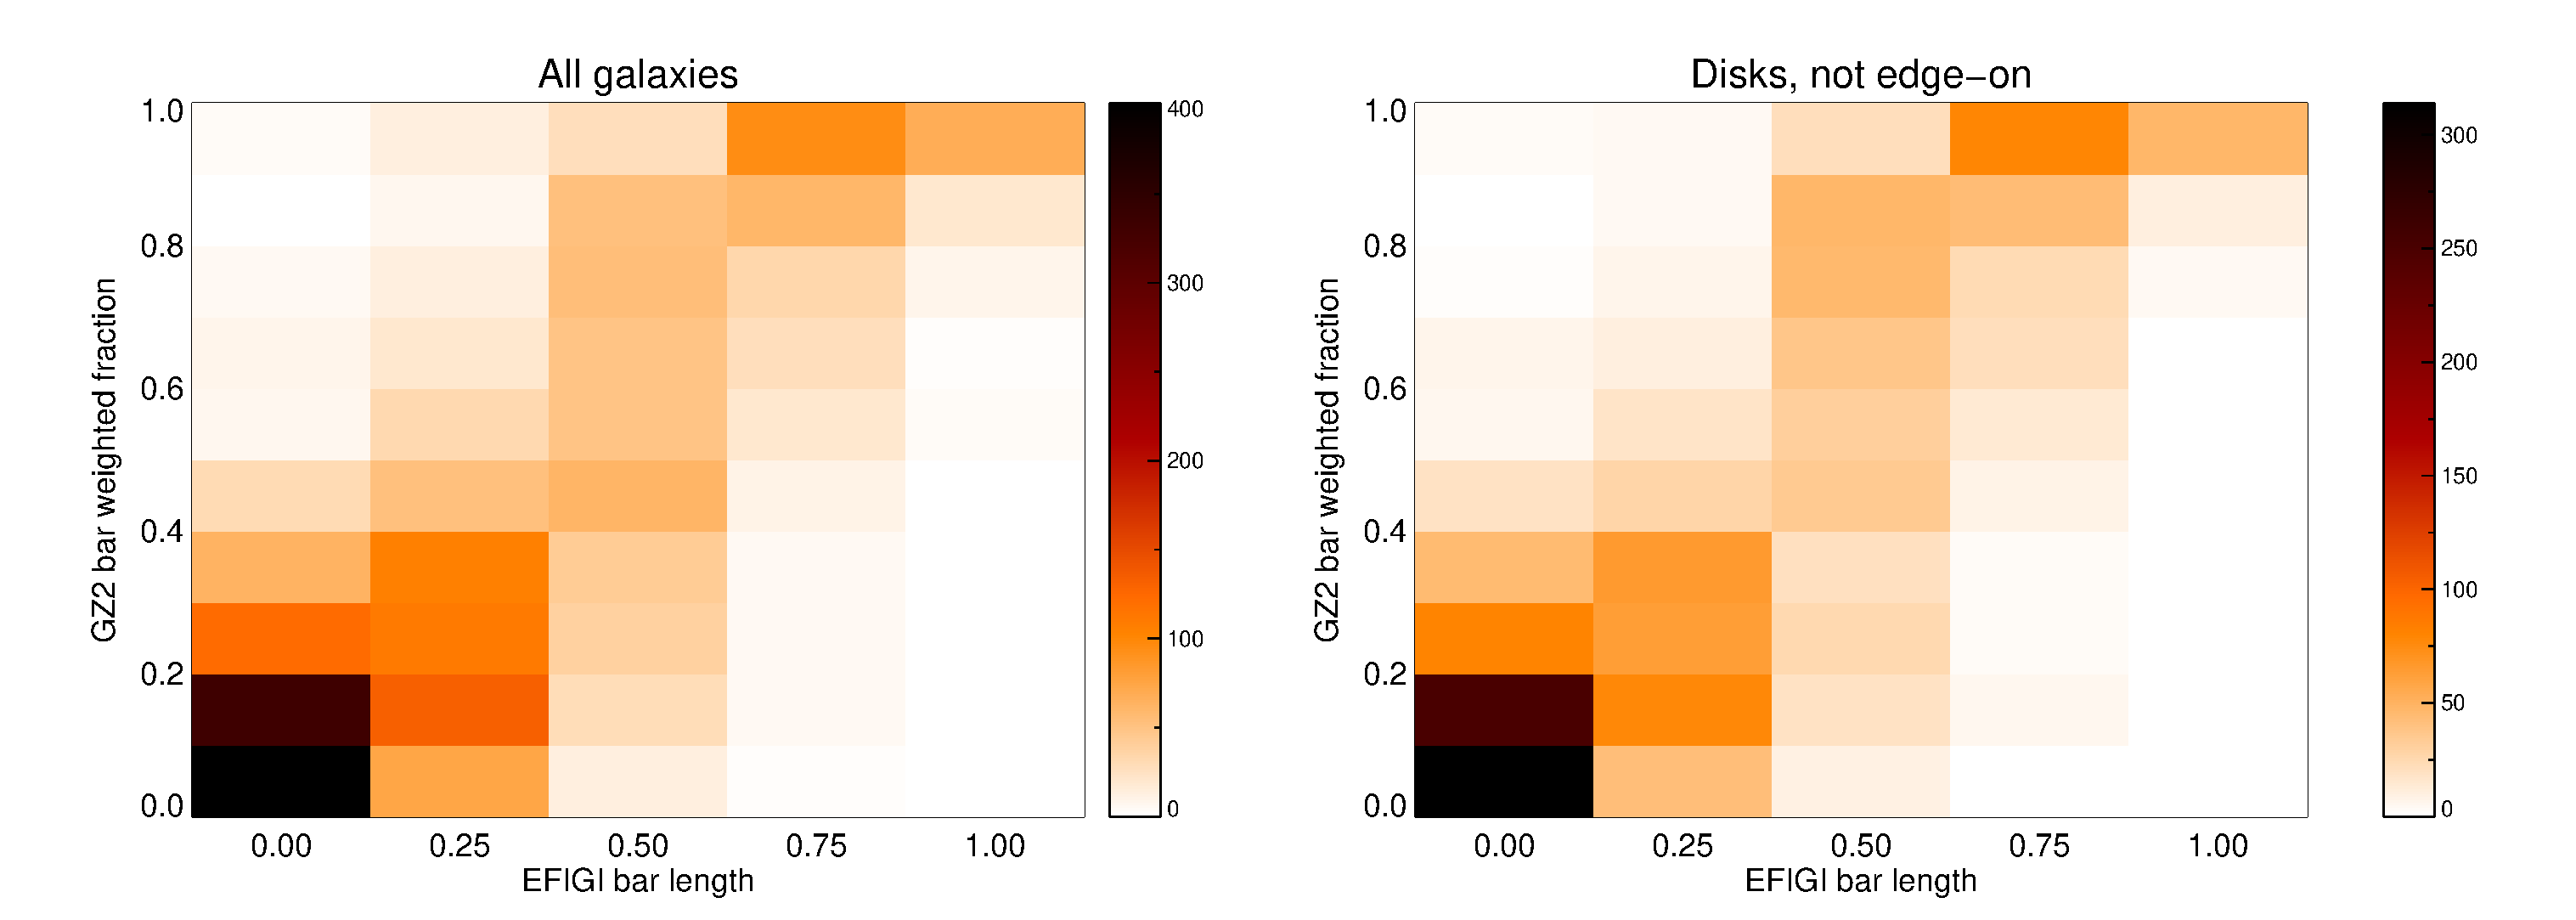
\includegraphics[angle=0,width=7.0in]{figures/efigi_bars.eps}
\caption{EFIGI bar length classifications compared to their GZ2 weighted fractions for the presence of a bar. Data on the left are for the 3,354 galaxies in both samples; the subset of 2,099 face-on galaxies is on the right. The dashed line is not a fit to the data, but is the one-to-one correlation. 
\label{fig-efigi_bars}}
\end{figure*}

\subsubsection{Bars}

GZ2 asks users to identify whether a bar is present in the galaxy. EFIGI's scale is based on bar length (not necessarily corresponding to strength) with respect to $D_{25}$, the decimal logarithm of the mean isophote diameter at a surface brightness of $\mu_B=25$~mag~arcsec$^{-2}$. A value of 1.0 (the strongest bar) extends more than half the length of $D_{25}$, while the median value of 0.5 would be about one-third the length of $D_{25}$. 

There is a strong correlation between the GZ2 weighted fractions for bars and the bar attribute strength from EFIGI (Figure~\ref{fig-efigi_bars}). 65\% of GZ2 galaxies in the overlap sample have no strong evidence for a bar (less than 0.3); of those, 77\% had EFIGI bar attributes of 0.0 and 94\% had 0.25 or less. For higher values of the GZ2 bar weighted fraction, the EFIGI attribute is slightly lower; the largest number of galaxies with GZ2 weighted fraction above 0.8 have EFIGI values of 0.75. The correlation coefficient between the variables is 0.51; if only face-on galaxies are considered, this increases to 0.75. 

If the \citet{mas11c} GZ2 weighted fraction of $\geq0.5$, at least 10 bar votes, and face-on galaxies is applied, then 98\% (646/660) galaxies overlapping with the EFIGI catalog have a bar attribute above 0. The mean EFIGI attribute (weighted by the confidence intervals) for galaxies barred by the \citet{mas11c} criteria is 0.62, indicating a selection preference toward medium-length bars, between one-third and one-half of $D_{25}$. 

The overall fraction of barred galaxies in EFIGI is 42\% (1439/3354); this is essentially unchanged if only face-on galaxies are considered (915/2099 = 44\%). This is significantly higher than the mean bar fraction of \citet{mas11c}, at 29.5\%, but consistent with results using automated ellipse-fitting techniques \citep{bar08,agu09}. The higher fraction in EFIGI is due to the contributions of galaxies with bar length attributes of 0.25, the majority of which have GZ2 weighted fractions below 0.5. If only EFIGI galaxies at 0.5 and above are considered to be barred, then the bar fraction falls to 17\%. Only some of the galaxies in the 0.25 EFIGI bin are being classified by the GZ2 users as barred; since \citet{bai11} defines this as a ``barely visible'' bar, it may be expected that less than half of GZ2 users would have detected it. 

\citet{mas11c} suggest in their paper that trends of bar fraction should ideally be discussed in the context of large or strong bars; an EFIGI cut of 0.5 or above would likely suit this philosophy best. 

\subsubsection{Arm curvature}

\begin{figure*}
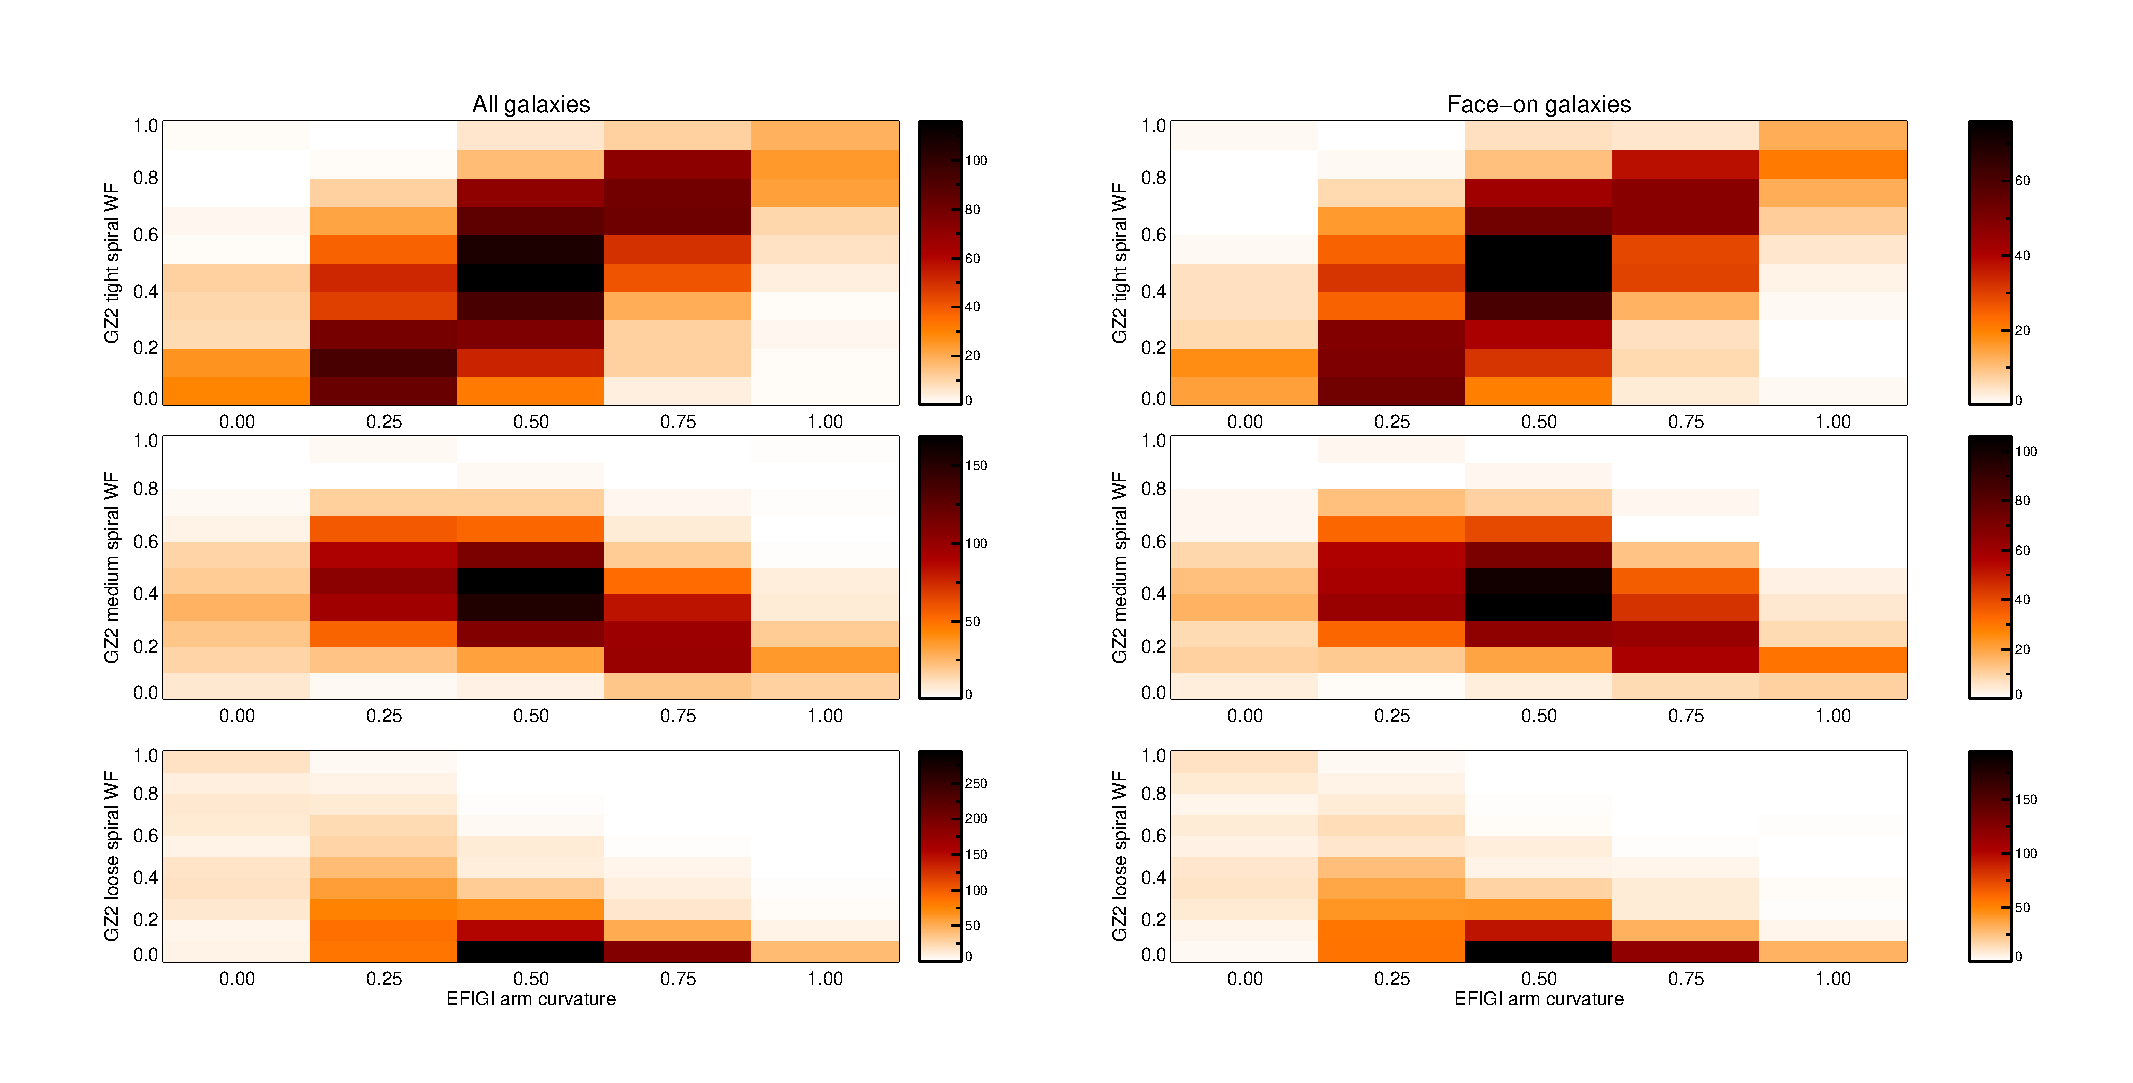
\includegraphics[angle=0,width=7.0in]{figures/efigi_arm_curvature.eps}
\caption{EFIGI arm curvature classifications compared to their GZ2 weighted fractions for the presence of a bar. Data on the left are for the 3,411 galaxies in both samples; the subset of 2,099 face-on galaxies is on the right. Dashed lines on the top and bottom pairs of plots show the one-to-one correlation, a Gaussian with $\mu=0.5$ and $\sigma=0.25$, and the one-to-one anti-correlation, respectively. 
\label{fig-efigi_arms}}
\end{figure*}

EFIGI measures the arm curvature of each galaxy, with classifications very similar to the ``tightness of spiral arms'' question (Task 10) in GZ2. If both tasks and classifiers agree, one would expect galaxies with high GZ2 weighted fractions/votes for tight spirals to have EFIGI classifications at 0.75--1.0; GZ2 galaxies classified as medium spirals to be centered around 0.5; and loose spirals to have arm curvatures of 0.0--0.25. 

The EFIGI arm curvature classifications broadly follow the trends expected from matching targets with GZ2. The tight spiral weighted fraction follows the trend of the EFIGI arm curvature (Figure~\ref{fig-efigi_arms}). The Spearman's correlation coefficient for tight spirals is $\rho=0.62$. The medium spiral weighted fraction is clustered in the middle of the EFIGI values, where galaxies with the highest GZ2 weighted fraction have EFIGI values of 0.25--0.50, with $\rho=-0.26$. Loose spirals shows an anti-correlation ($\rho=-0.54$); very few galaxies have GZ2 weighted fractions above 0.5, but those which do have low EFIGI arm curvature values (0.0--0.25). 

Trends described above are quantitatively similar for both the full matching sample and for face-on galaxies only (right side of Figure~\ref{fig-efigi_arms}). Somewhat surprisingly, the distribution also appears similar if only considering galaxies with a mininum number of GZ2 votes on spiral winding arms. Lower limits of 5, 10, 20, and 30 votes produce the same patterns for all three categories. The correlation coefficient for both tight and medium spirals does decrease to $|\rho<0.2|$ if a 10-vote lower limit is applied. 

Most useful: look at high weighted fractions and high numbers of vote counts for the spiral winding category of choice. That might correlate most strongly with EFIGI values. 

EFIGI values are matched to specific pitch angles of the galaxy. For galaxies in which the GZ2 WF does not match the EFIGI, what is happening? Are the vote categories laterally skewed, are we not sensitive to weakest spirals, or is something else going on?

Not convinced that the face-on criterion is working. 

Change bar plot to single-panel version. Change right side of arm curvature to cuts on count and weighted vote fraction, show stronger correlations. Discuss the percentage of the total number of galaxies that this constitutes for the expanded GZ2 sample, and how many ``clean'' galaxies from the EFIGI criteria we might be able to extract (subject to bias at lower surface brightnesses).

\subsection{Huertas-Company - automated classifications}

\begin{figure*}
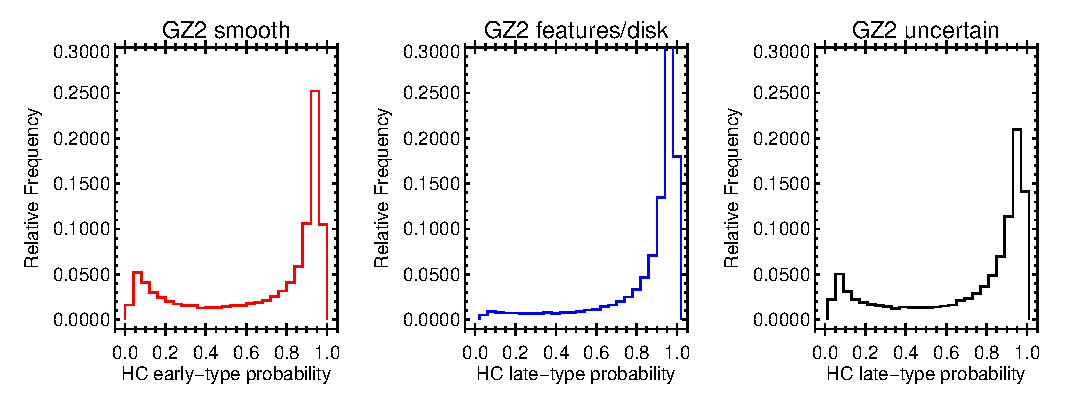
\includegraphics[angle=0,width=7.0in]{figures/hc_histogram.eps}
\caption{Left: distribution of HC early-type probabilities for galaxies with Task 01 ``smooth'' weighted fraction above 0.8. Middle: distribution of HC late-type probabilities for galaxies with Task 01 ``features or disk'' weighted fraction above 0.8. Right: HC late-type probabilities for uncertain galaxies ($p<0.8$ for all responses to Task 01). 
\label{fig-hc_histogram}}
\end{figure*}

\citet{hue11} published a study in which they used training sets of galaxies to create artificial classifications, and then compared the results to GZ1. There have been no comparisons to GZ2; however, the broad nature of their probabilities (four broad morphological categories) are not suited for the fine structure questions such as bar and spiral number. 

The classified sample of HC is the SDSS DR7 spectroscopic sample, limited to galaxies with $z<0.25$ with good photometric data and clean spectra. Their total of 698,420 galaxies is approximately the size of the GZ2 sample, which has a similar redshift range. The primary difference between the samples is that the HC sample goes to fainter depths, with more than 400,000 galaxies below the GZ2 limit of $r>17$. The algorithm for classification is implemented using support vector machine software that tries to find boundaries between points in $N$-dimensional space. The training set for galaxy morphology is the 2,253 galaxies in \citet{fuk07}, classified by T-Type. Each galaxy has a probability of being in one of four subclasses: E, S0, Sab, and Scd. 

\citet{hue11} directly compare their results to the GZ1 sample from \citet{lin11}. They find that robust classifications in GZ1 (flagged in our clean sample as being either confirmed ellipticals or spirals) have median probabilities of 0.92 according to their algorithm, indicating that sure GZ1 classifications are also sure in their catalog. They also find a (but not strictly linear) relationship between the GZ1 debiased vote fraction and the HC probabilities. This is one of the first independent confirmations that the vote fractions may be related to the actual {\em probability} of a galaxy possessing a particular morphology. 

HC also compare their results to the NA10 data, most of which are not included in the HC training sample. They find a good correlation between the NA10 T-Types and the HC probabilities, especially for ellipticals and Scd spirals. S0 galaxies are more difficult to separate; for the NA10 lenticulars, HC11 give only a 0.4 probability of S0, with 0.32 of elliptical and 0.2 of being Sab. Sab galaxies have an average probability of 0.55 being an Sab in HC, but also 0.15 of being S0 or Scd. The HC algorithm is thus very good at identifying galaxies at the extreme ends of the Hubble tuning fork, but have larger amounts of overlapping probabilities for intermediate states. 

Since the GZ2 galaxies are a subset of the GZ1 sample, the results are expected to be similar to those described in \citet{hue11}. Figure~\ref{fig-hc_histogram} shows the distributions of the HC early- and late-type probabilities for GZ2 galaxies robustly identified ($p > 0.8$) as either smooth or having features/disks. The median HC early-type probability for GZ2 ellipticals is 0.85, and the late-type probability for GZ2 spirals is 0.95. This confirms the result that robust classifications in Galaxy Zoo agree with the automated algorithm. 

An exception to this is a population of galaxies classified as ``smooth'' by GZ2 users, but which have very low early-type probabilities from HC (the bump on the left side of the first panel in Figure~\ref{fig-hc_histogram}). The average GZ2 vote fraction for these galaxies is consistent with those with high early-type probabilities -- these galaxies are not marginally classified as ellipticals in GZ2. The roundness of the galaxy (Task 07 in GZ2) seems to play some role, as the low-HC smooth galaxies have fewer round galaxies and many more ``cigar-shaped'' galaxies in this sample. A high axial ratio might have trained the HC algorithm to infer the existence of a disk; the absence of any obvious spiral features or bulge/disk separation (verified by eye in a small subsample of the imaages) lead GZ2 users to categorize them as ``smooth''. There is a clear dependence on apparent magnitude; the lower peak disappears if only galaxies with $r < 16$ are plotted. The lower peak is also significantly bluer than the higher peak, with respective colors of $(g-r)=0.67$ and $(g-r)=0.97$. Since the SVM method does include SDSS colors as a parameter, we conjecture that the low HC early-type probability is in part due to the fact that they are blue, in addition to morphological features such as shape and concentration. It would be interesting to see what fraction of the blue ellipticals \citep{sch09} fall in this peak. 

The right panel of Figure~\ref{fig-hc_histogram} shows the distribution of ``unclassified'' galaxies, for which none of the reponses for Task 01 had a weighted fraction above 0.8. The HC probability for these galaxies is bimodal, with the larger fraction classified as HC late-type and a smaller fraction as HC early-type. 

Figure~\ref{fig-hc_gz2} plots the HC probability values against the GZ2 vote fraction for both smooth and feature/disk galaxies, similar to Figure~8 in \citet{hue11}. Significant excesses are seen at the lower left and upper right corners for both samples, confirming the earlier result that robust classifications using both methods tend to agree. The relationship of the HC probability to GZ2 vote fraction, however, seems distinctly non-linear and significantly different from the relationship shown in \citet{hue11}. Galaxies with low HC early-type probabilities show no strong correlation with the GZ2 weighted fraction, resulting in the vertical stripe in Figure~\ref{fig-hc_gz2}. Intermediate values of the HC probabilities are typically classified by GZ2 users as ``smooth'', with a concentration at the highest HC early-type probabilities. It should be noted that without GZ2 debiasing, the two panels in Figure~\ref{fig-hc_gz2} are essentially mirror images of each other (since $p_{HC,early} + p_{HC,late} \equiv 1$ and the GZ2 weighted fractions only have marginal contributions from either the star/artifact response or downweighting of inconsistent users). 

Splitting the HC morphology types into the E, S0, Sab, and Scd subclasses, Figure~\ref{fig-hc_gz2_subclass} shows the correlations to the GZ2 weighted fractions. While the direction of the correlation is the same as seen in Figures~9 and 10 in \citet{hue11}, the behavior at the extrema is quite different. The debiased GZ1 data shows a strong cluster of low-HC and low-GZ probabilities for all four subclasses; no such cluster is seen in any of the plots in Figure~\ref{fig-hc_gz2_subclass}. Furthermore, high HC probabilities have the lowest fraction of galaxies in the GZ1 published data, where our plots show a concentration of galaxies along the high end for both P(E) and P(S0). It should be investigated whether the scaling on these sets of figures is truly plotting the same value. 

\begin{itemize}
	\item Check how the presence of a bar affects the HC classifications
	\item Since T-Types seem to be most strongly correlated with bulge prominence, plot these against each other. 
\end{itemize}

\begin{figure*}
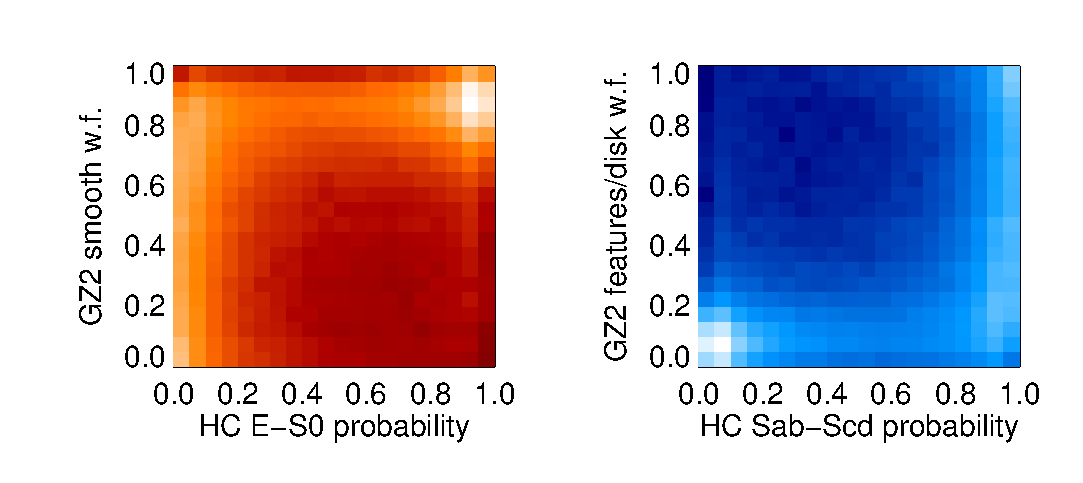
\includegraphics[angle=0,width=7.0in]{figures/hc_gz2.eps}
\caption{Left: GZ2 smooth weighted fraction as a function of \citet{hue11} early-type probability. Right: GZ2 features/disk weighted fraction as a function of HC late-type probability. Whiter values in both indicate a larger fraction of galaxies in that bin (logarithmic scale).
\label{fig-hc_gz2}}
\end{figure*}

\begin{figure*}
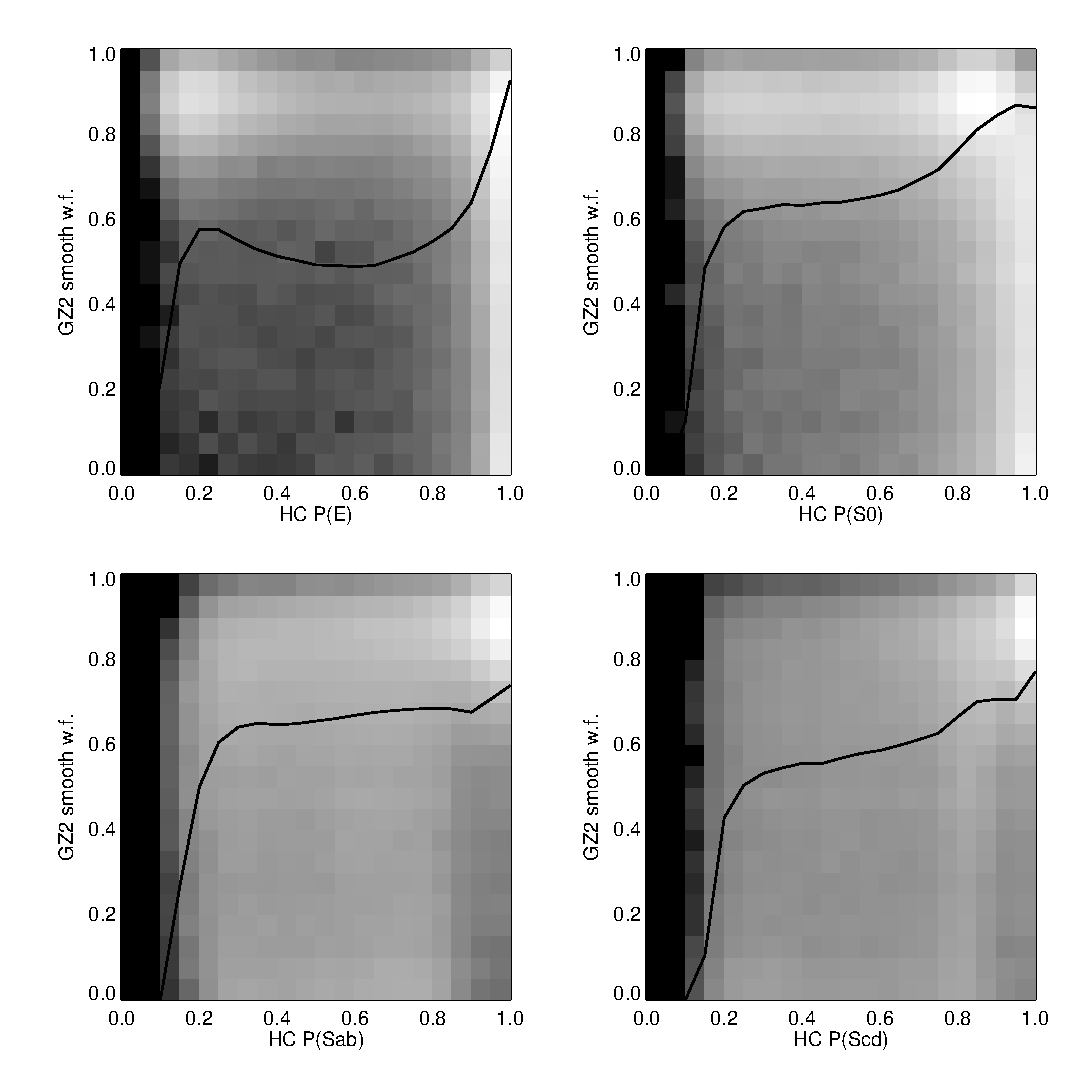
\includegraphics[angle=0,width=6.0in]{figures/hc_gz2_subclass.eps}
\caption{Left: GZ2 smooth weighted fraction as a function of \citet{hue11} early-type probability. Right: GZ2 features/disk weighted fraction as a function of HC late-type probability. Whiter values in both indicate a larger fraction of galaxies in that bin (logarithmic scale).
\label{fig-hc_gz2_subclass}}
\end{figure*}



\section{Galaxy Wars}\label{sec_galaxywars}
\section{Astronomy}\label{sec_astronomy}

\section{Conclusions}\label{sec_conclusions}

%%%%%%%%%%%%
%%% ACKNOWLEDGMENTS
%%%%%%%%%%%%

%\acknowledgments
%

%\clearpage

%%%%%%%%%%%%
%%% BIBLIOGRAPHY
%%%%%%%%%%%%

\bibliography{mn-jour,kwrefs}

\bsp

\newpage
\clearpage
\tabletypesize{\scriptsize}
\begin{deluxetable}{lccrrrr}
\tablecolumns{16}
\tablewidth{0pc}
\tablecaption{GZ2 weighted vote fractions for the main and Stripe~82 normal-depth samples \label{tbl-stripe82}}
\tabletypesize{\scriptsize}
\tablehead{
 & \multicolumn{2}{c}{\underline{Mean weighted vote fraction}} & \multicolumn{2}{c}{\underline{Number of galaxies}} & \multicolumn{2}{c}{\underline{Sample comparison}} \\
\colhead{User task and answer} & 
\colhead{Main} & 
\colhead{Stripe 82} & 
\colhead{Main} & 
\colhead{Stripe 82} &
\colhead{$f_m - f_s$} & 
\colhead{$f_m/f_s$} 
}
\small
\startdata
T01\_SMOOTH\_OR\_FEATURES\_A01\_SMOOTH                      &      0.642 &      0.613 &     273783 &       8437 &       0.029 &       1.048 \\
T01\_SMOOTH\_OR\_FEATURES\_A02\_FEATURES\_OR\_DISK          &      0.325 &      0.352 &     273783 &       8437 &      -0.027 &       0.924 \\
T01\_SMOOTH\_OR\_FEATURES\_A03\_STAR\_OR\_ARTIFACT          &      0.033 &      0.036 &     273783 &       8437 &      -0.003 &       0.924 \\
T02\_EDGEON\_A04\_YES                                       &      0.234 &      0.229 &     118147 &       4110 &       0.005 &       1.020 \\
T02\_EDGEON\_A05\_NO                                        &      0.766 &      0.771 &     118147 &       4110 &      -0.005 &       0.994 \\
T03\_BAR\_A06\_BAR                                          &      0.287 &      0.292 &      87647 &       3077 &      -0.004 &       0.986 \\
T03\_BAR\_A07\_NO\_BAR                                      &      0.713 &      0.708 &      87647 &       3077 &       0.004 &       1.006 \\
T04\_SPIRAL\_A08\_SPIRAL                                    &      0.660 &      0.674 &      87621 &       3077 &      -0.014 &       0.980 \\
T04\_SPIRAL\_A09\_NO\_SPIRAL                                &      0.340 &      0.326 &      87621 &       3077 &       0.014 &       1.042 \\
T05\_BULGE\_PROMINENCE\_A10\_NO\_BULGE                      &      0.129 &      0.114 &      87608 &       3076 &       0.015 &       1.129 \\
T05\_BULGE\_PROMINENCE\_A11\_JUST\_NOTICEABLE               &      0.479 &      0.491 &      87608 &       3076 &      -0.012 &       0.976 \\
T05\_BULGE\_PROMINENCE\_A12\_OBVIOUS                        &      0.321 &      0.333 &      87608 &       3076 &      -0.011 &       0.966 \\
T05\_BULGE\_PROMINENCE\_A13\_DOMINANT                       &      0.070 &      0.062 &      87608 &       3076 &       0.008 &       1.134 \\
T06\_ODD\_A14\_YES                                          &      0.199 &      0.185 &     273636 &       8391 &       0.014 &       1.073 \\
T06\_ODD\_A15\_NO                                           &      0.801 &      0.815 &     273636 &       8391 &      -0.014 &       0.983 \\
T07\_ROUNDED\_A16\_COMPLETELY\_ROUND                        &      0.330 &      0.326 &     229974 &       6956 &       0.005 &       1.014 \\
T07\_ROUNDED\_A17\_IN\_BETWEEN                              &      0.496 &      0.501 &     229974 &       6956 &      -0.004 &       0.991 \\
T07\_ROUNDED\_A18\_CIGAR\_SHAPED                            &      0.173 &      0.174 &     229974 &       6956 &      -0.000 &       0.999 \\
T08\_ODD\_FEATURE\_A19\_RING                                &      0.147 &      0.178 &      72439 &       2114 &      -0.031 &       0.827 \\
T08\_ODD\_FEATURE\_A20\_LENS\_OR\_ARC                       &      0.045 &      0.040 &      72439 &       2114 &       0.005 &       1.122 \\
T08\_ODD\_FEATURE\_A21\_DISTURBED                           &      0.121 &      0.125 &      72439 &       2114 &      -0.003 &       0.973 \\
T08\_ODD\_FEATURE\_A22\_IRREGULAR                           &      0.177 &      0.170 &      72439 &       2114 &       0.007 &       1.039 \\
T08\_ODD\_FEATURE\_A23\_OTHER                               &      0.282 &      0.245 &      72439 &       2114 &       0.037 &       1.152 \\
T08\_ODD\_FEATURE\_A24\_MERGER                              &      0.212 &      0.209 &      72439 &       2114 &       0.003 &       1.015 \\
T08\_ODD\_FEATURE\_A38\_DUST\_LANE                          &      0.016 &      0.034 &      72439 &       2114 &      -0.018 &       0.475 \\
T09\_BULGE\_SHAPE\_A25\_ROUNDED                             &      0.538 &      0.567 &      21496 &        746 &      -0.029 &       0.948 \\
T09\_BULGE\_SHAPE\_A26\_BOXY                                &      0.103 &      0.096 &      21496 &        746 &       0.007 &       1.077 \\
T09\_BULGE\_SHAPE\_A27\_NO\_BULGE                           &      0.359 &      0.338 &      21496 &        746 &       0.022 &       1.065 \\
T10\_ARMS\_WINDING\_A28\_TIGHT                              &      0.370 &      0.392 &      55800 &       2052 &      -0.022 &       0.943 \\
T10\_ARMS\_WINDING\_A29\_MEDIUM                             &      0.417 &      0.405 &      55800 &       2052 &       0.011 &       1.028 \\
T10\_ARMS\_WINDING\_A30\_LOOSE                              &      0.214 &      0.203 &      55800 &       2052 &       0.011 &       1.054 \\
T11\_ARMS\_NUMBER\_A31\_1                                   &      0.074 &      0.067 &      55805 &       2053 &       0.008 &       1.117 \\
T11\_ARMS\_NUMBER\_A32\_2                                   &      0.501 &      0.478 &      55805 &       2053 &       0.023 &       1.048 \\
T11\_ARMS\_NUMBER\_A33\_3                                   &      0.093 &      0.098 &      55805 &       2053 &      -0.005 &       0.950 \\
T11\_ARMS\_NUMBER\_A34\_4                                   &      0.038 &      0.043 &      55805 &       2053 &      -0.005 &       0.884 \\
T11\_ARMS\_NUMBER\_A36\_MORE\_THAN\_4                       &      0.030 &      0.033 &      55805 &       2053 &      -0.002 &       0.934 \\
T11\_ARMS\_NUMBER\_A37\_CANT\_TELL                          &      0.263 &      0.281 &      55805 &       2053 &      -0.019 &       0.934 \\
\enddata
\tablecomments{Data for each task is only for galaxies with at least 10 total responses to the classification question.}
\end{deluxetable}

\label{lastpage}

\end{document}
